\section{Monitoring Application}
\label{mobile-application}
We hit another mother lode. This time we have to bring all the MQTT client implementation onto a mobile application. Most of the idea will be the same as what have been proposed for the gateway. I will spend more time discuss about modern mobile application development rather than digging into the MQTT. Let warm up with the Jetpack components.

\subsection{Jetpack Architecture}
Until recently, Google did not recommend a specific approach to building Android apps other than to provide tools and development kits while letting developers decide what worked best for a particular project or individual programming style. That changed in 2017 with the introduction of the Android Architecture Components which, in turn, became part of Android Jetpack when it was released in 2018. Android Jetpack consists of Android Studio, the Android Architecture Components and Android Support 
Library together with a set of guidelines that recommend how an Android App should be structured. The 
Android Architecture Components are designed to make it quicker and easier both to perform common tasks 
when developing Android apps while also conforming to the key principle of the architectural guidelines.

There are many components that makes up the Jetpack architecture, and our mobile application only use three: the \textit{ViewModel}, the \textit{Data Binding}, and the \textit{Navigation Graph}. They will be discussed shortly in upcoming sub-sections. Before moving on, it is important to understand the Jetpack approach to app development is not mandatory. While highlighting some of the shortcoming of other techniques that have gained popularity of the years, Google stopped short of completely condemning those approaches to app development. Google appears to be taking the position that while there is no right or wrong way to develop an app, there is a recommended way.

\subsubsection{Traditional Architecture}
An Android project typically consists of a single activity which contains all of the code for presenting and managing the user interface together with the back-end logic of the app. Up until the introduction of Jetpack, the most common architecture followed this paradigm with apps consisting of multiple activities (one for each screen within the app) with each activity class to some degree mixing user interface and back-end code.

This approach led to a range of problems related to the lifecycle of an app (for example an activity is destroyed and recreated each time the user rotates the device leading to the loss of any app data that had not been saved to some form of persistent storage) as well as issues such as inefficient navigation involving launching a new activity for each app screen accessed by the user.

At the most basic level, Google now advocates single activity apps where different screens are loaded as content within the same activity. Modern architecture guidelines also recommend separating different areas of responsibility within an app into entirely separate modules (a concept Google refers to as “separation of concerns”). One of the keys to this approach is the \textit{ViewModel} component.

\subsubsection{The ViewModel Component}
The purpose of ViewModel is to separate the user interface-related data model and logic of an app from the code responsible for actually displaying and managing the user interface and interacting with the operating system (Figure \ref{fig:viewmodel}). When designed in this way, an app will consist of one or more \textbf{UI Controllers}, such as an activity, together with ViewModel instances responsible for handling the data needed by those controllers.

In effect, the ViewModel only knows about the data model and corresponding logic. It knows nothing about the user interface and makes no attempt to directly access or respond to events relating to views within the user interface. When a UI controller needs data to display, it simply asks the ViewModel to provide it. Similarly, when the user enters data into a view within the user interface, the UI controller passes it to the ViewModel for handling.

This separation of responsibility addresses the issues relating to the lifecycle of UI controllers. Regardless of how many times a UI controller is recreated during the lifecycle of an app, the ViewModel instances remain in memory thereby maintaining data consistency. A ViewModel used by an activity, for example, will remain in memory until the activity completely finishes which, in the single activity app, is not until the app exits.

\begin{figure}
    \centering
    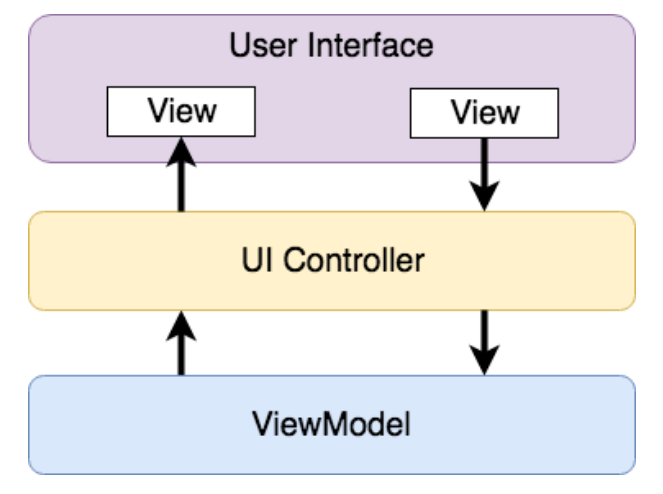
\includegraphics[scale=0.5]{screenshots/viewmodel.png}
    \caption{Jetpack Component - ViewModel}
    \label{fig:viewmodel}
\end{figure}

\subsubsection{LiveData and Data Binding}
Consider an app that displays realtime data such as the current price of a financial stock. There are only two ways that the UI controller can ensure that the latest data is displayed in the user interface. One option is for the controller to continuously check with the ViewModel to find out if the data has 
changed since it was last displayed. The problem with this approach, however, is that it is inefficient. To maintain the realtime nature of the data feed, the UI controller would have to run on a loop, continuously checking for the data to change.

A better solution would be for the UI controller to receive a notification when a specific data item within a ViewModel changes. This is made possible by using the \textit{LiveData} component. LiveData is a data holder that allows a value to become \textbf{observable} . In basic terms, an observable object has the ability to notify other objects when changes to its data occur thereby solving the problem of making sure that the user interface always matches the data within the ViewModel.

Another of the key advantages of using LiveData is that it is aware of the lifecycle state of its observers. If, for example, an activity contains a LiveData observer, the corresponding LiveData object will know when the activity’s lifecycle state changes and respond accordingly. If the activity is paused (perhaps the app is put into the background), the LiveData object will stop sending events to the observer. If the activity has just started or resumes after being paused, the LiveData object will send a LiveData event to the observer so that the activity has the most up to date value. Similarly, the LiveData instance will know when the activity is destroyed and remove the observer to free up resources.

Android Jetpack includes the Data Binding Library which allows data in a ViewModel to be mapped directly to specific views within the XML user interface layout file. Data binding allows the LiveData value stored in the ViewModel to be referenced directly within the XML layout file avoiding the need to write code to keep the layout views updated. Figure \ref{fig:data-binding} illustrates the idea.

\begin{figure}
    \centering
    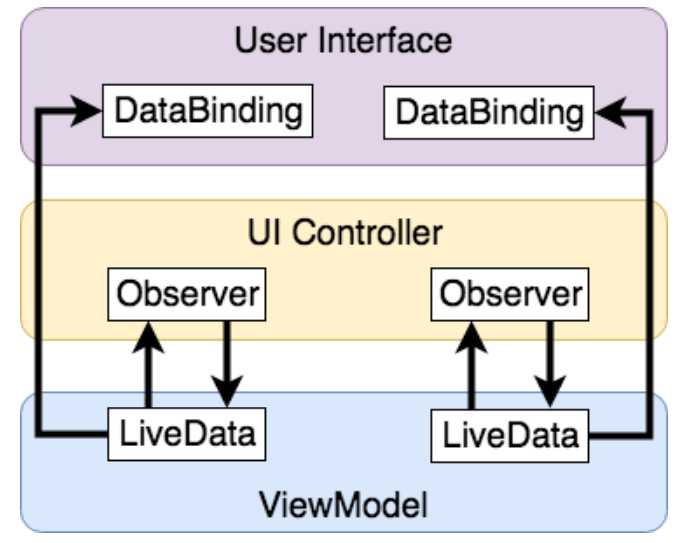
\includegraphics[scale=0.5]{screenshots/data binding.png}
    \caption{Jetpack Component - Data Binding}
    \label{fig:data-binding}
\end{figure}

\subsubsection{Navigation Graph}
Prior to the introduction of Android Jetpack, the implementation of navigation within an app was largely a manual coding process with no easy way to view and organize potentially complex navigation paths. This situation has improved considerably, however, with the introduction of the Android Navigation Architecture Component combined with support for navigation graphs in Android Studio.

A navigation graph is an XML file which contains the destinations that will be included in the app navigation. In addition to these destinations, the file also contains navigation actions that define navigation between destinations, and optional arguments for passing data from one destination to another. Android Studio includes a navigation graph editor that can be used to design graphs and implement actions either visually or by manually editing the XML. Figure \ref{fig:navigation-graph} shows the navigation graph of our mobile application.

\begin{figure}
    \centering
    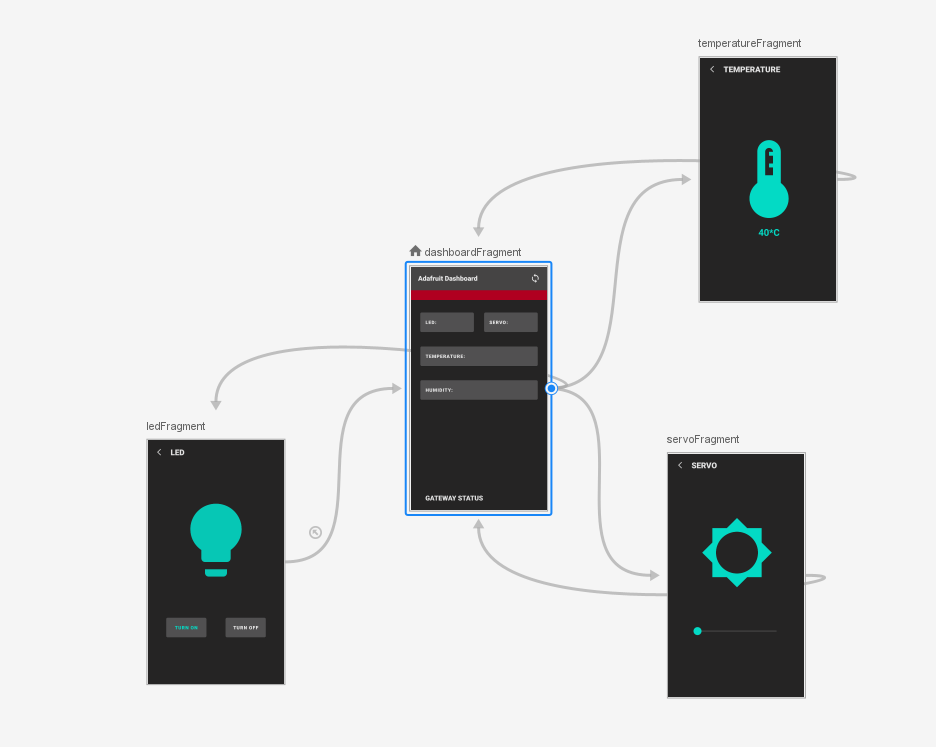
\includegraphics[scale=0.5]{screenshots/navigation_graph.png}
    \caption{Jetpack Component - Navigation Graph}
    \label{fig:navigation-graph}
\end{figure}

\subsection{MQTT in Mobile Application}
It would a pain if the implementation of our Android application is presented here. As I stated before, the project is hosted in this Github \href{https://github.com/hescul/adafruit-simple-iot}{\textcolor{blue}{repository}}, so it will be much more practical (and realistic) to pay it a visit. I will devote this section to explain how I achieve the MQTT protocol in an mobile app, together with modern components that we have come through. Listing \ref{code:mobile-main} shows the SIMPLIFIED version of the main activity class of our mobile app.
\begin{lstlisting}[language=Java, caption= Main Activity, escapeinside={(*}{*)}, label=code:mobile-main]
public class MainActivity extends AppCompatActivity
{
    // private fields
    // -----
    private MqttAndroidClient _client;
    private MqttConnectOptions _connectOptions;
    private DisconnectedBufferOptions _disconnectedBufferOptions;

    private DashboardViewModel _dashboardViewModel;


    // lifecycle methods
    // -----
    @Override
    protected void onCreate(@Nullable Bundle savedInstanceState) {
        super.onCreate(savedInstanceState);

        // inflate root view for this activity using view bing library
        setContentView(ActivityMainBinding.inflate(getLayoutInflater()).getRoot());

        // setup view model for fragments
        _dashboardViewModel = new ViewModelProvider(this).get(DashboardViewModel.class);

        // initialize and connect a client
        initClient();       (*\label{code:mobile-main:init}*)
        connectClient();    (*\label{code:mobile-main:connect}*)
    }

    @Override
    protected void onDestroy() {
        super.onDestroy();
        disconnectClient(); (*\label{code:mobile-main:disconnect}*)
    }

    // mqtt utilities
    // -----
    private void initClient() {
        final String serverURI = BrokerConfig.AUTH_CONTEXT + "://" + BrokerConfig.HOST_NAME + ':' + BrokerConfig.HOST_PORT;
        _client = new MqttAndroidClient(getApplicationContext(), serverURI, ClientConfig.CLIENT_ID);
        setupClient();
        setupCallback();
    }

    private void setupCallback() {
        _client.setCallback(new MqttCallbackExtended() {
            @Override
            public void connectComplete(boolean reconnect, String serverURI) {
                Timber.tag(logTag).d("Connected successfully: %s", serverURI);
            }

            @Override
            public void connectionLost(Throwable cause) {
                if (cause != null) {
                    Timber.tag(logTag).e("Lost connection to broker: %s", cause.getMessage());
                    _dashboardViewModel.setErrorMessage(cause.getMessage() + _dashboardViewModel.errorSuffix);
                    _dashboardViewModel.setConnected(false);
                }
            }

            @Override
            public void messageArrived(String topic, MqttMessage message) {
                Timber.tag(logTag).d("Received '%s' from %s", message, topic.substring(topic.indexOf('.') + 1));
                if (topic.contains(ClientConfig.SUBSCRIBE_TOPICS[ClientConfig.TOPICS.LED.ordinal()])) {             // led message
                    _dashboardViewModel.setLedStatus(message.toString());
                }
                else if (topic.contains(ClientConfig.SUBSCRIBE_TOPICS[ClientConfig.TOPICS.SERVO.ordinal()])) {      // servo message
                    _dashboardViewModel.setServoValue(message.toString());
                }
                else if (topic.contains(ClientConfig.SUBSCRIBE_TOPICS[ClientConfig.TOPICS.TEMPERATURE.ordinal()])) {// temperature message
                    _dashboardViewModel.setTemperatureValue(message.toString());
                }
                else if (topic.contains(ClientConfig.SUBSCRIBE_TOPICS[ClientConfig.TOPICS.HUMIDITY.ordinal()])) {   // humidity message
                    _dashboardViewModel.setHumidityValue(message.toString());
                }
                else if (topic.contains(ClientConfig.SUBSCRIBE_TOPICS[ClientConfig.TOPICS.STATUS.ordinal()])) {     // status message
                    _dashboardViewModel.setGtwStatus(message.toString());
                }
            }

            @Override
            public void deliveryComplete(IMqttDeliveryToken token) {
                try {
                    if (!token.getMessage().toString().isEmpty()) {
                        Timber.tag("mqtt").d("Delivered successfully (messageID = %d)", token.getMessageId());
                    }
                } catch (MqttException e) {
                    e.printStackTrace();
                }
            }
        });

    }

    private void setupClient() {
        // setup connection options
        _connectOptions = new MqttConnectOptions();
        _connectOptions.setUserName(BrokerConfig.USERNAME);
        _connectOptions.setPassword(BrokerConfig.PASSWORD.toCharArray());
        _connectOptions.setAutomaticReconnect(false);
        _connectOptions.setCleanSession(true);

        // setup disconnected buffer options
        _disconnectedBufferOptions = new DisconnectedBufferOptions();
        _disconnectedBufferOptions.setBufferEnabled(true);
        _disconnectedBufferOptions.setBufferSize(100);
        _disconnectedBufferOptions.setPersistBuffer(false);
        _disconnectedBufferOptions.setDeleteOldestMessages(false);
    }

    private void connectClient() {
        _dashboardViewModel.setConnecting(true);
        try {
            _client.connect(_connectOptions, null, new IMqttActionListener() {
                @Override
                (*\label{code:mobile-main:on-success}*)
                public void onSuccess(IMqttToken asyncActionToken) {
                    _client.setBufferOpts(_disconnectedBufferOptions);
                    subscribe();
                    fetchLatest();
                    _dashboardViewModel.setConnected(true);
                    _dashboardViewModel.setConnecting(false);
                }

                @Override
                public void onFailure(IMqttToken asyncActionToken, Throwable exception) {
                    Timber.tag(logTag).e("%s failed to reach %s: %s", ClientConfig.CLIENT_ID, BrokerConfig.HOST_NAME, exception.getMessage());
                    _dashboardViewModel.setErrorMessage(exception.getMessage() + _dashboardViewModel.errorSuffix);
                    _dashboardViewModel.setConnected(false);
                    _dashboardViewModel.setConnecting(false);
                }
            });
        } catch (MqttException e) {
            e.printStackTrace();
        }
    }

    private void disconnectClient() {
        if (_client.isConnected()) {
            try {
                IMqttToken token = _client.disconnect();
                token.setActionCallback(new IMqttActionListener() {
                    @Override
                    public void onSuccess(IMqttToken asyncActionToken) {
                        Timber.tag(logTag).d("%s disconnected successfully", ClientConfig.CLIENT_ID);
                    }

                    @Override
                    public void onFailure(IMqttToken asyncActionToken, Throwable exception) {
                        Timber.tag(logTag).e("%s failed to disconnect: %s", ClientConfig.CLIENT_ID, exception.getMessage());
                    }
                });

            } catch (MqttException e) {
                e.printStackTrace();
            }
        }
    }

    private void subscribe() {

        for (String topic : ClientConfig.SUBSCRIBE_TOPICS) {
            try {
                String realTopic = String.format("%s/feeds/%s.%s", BrokerConfig.USERNAME, ClientConfig.GROUP_KEY, topic);
                _client.subscribe(realTopic, 0, null, new IMqttActionListener() {
                    @Override
                    public void onSuccess(IMqttToken asyncActionToken) {

                    }

                    @Override
                    public void onFailure(IMqttToken asyncActionToken, Throwable exception) {
                        Timber.tag(logTag).e("Failed to subscribe to %s", topic);
                    }
                });
            } catch (MqttException e) {
                e.printStackTrace();
            }
        }
    }

    private void fetchLatest() {
        for (String topic : ClientConfig.SUBSCRIBE_TOPICS) {
            publish(String.format("%s/get", topic), "");
        }
    }
    private void fetchLatest(String topic) {
        publish(String.format("%s/get", topic), "");
    }

    private int publish(String topic, String msg) {
        String realTopic = String.format("%s/feeds/%s.%s", BrokerConfig.USERNAME, ClientConfig.GROUP_KEY, topic);
        int msgID = 0;
        try {
            IMqttToken token = _client.publish(realTopic, msg.getBytes(StandardCharsets.UTF_8), 0, false);
            token.setActionCallback(new IMqttActionListener() {
                @Override
                public void onSuccess(IMqttToken asyncActionToken) {

                }

                @Override
                public void onFailure(IMqttToken asyncActionToken, Throwable exception) {
                    Timber.tag("mqtt").e("Failed to publish %s to %s",msg ,topic);
                }
            });
            msgID = token.getMessageId();
        } catch (MqttException e) {
            e.printStackTrace();
        }
        return msgID;
    }
}
\end{lstlisting}
All the MQTT-things are gathered inside this class. The implementation may look different from that of in Python, but the overall idea is the same. When the host activity is created, we make the 2 calls to the \texttt{initClient()} and \texttt{connectClient()} function. They respectively construct an MQTT client instance and establish a connection for it to the broker (line \ref{code:mobile-main:init} and line \ref{code:mobile-main:connect}). When the activity get destroyed, we also disconnect the client from the server, as shown at line \ref{code:mobile-main:disconnect}. Another point that need pointed out is that we override the callback \texttt{onSuccess()} at line \ref{code:mobile-main:on-success} to have it subscribe to required topics and fetch latest data for us each time we successfully connect to the server.

And I think that's the main idea. Again, all the Android-related things can be found at this Github \href{https://github.com/hescul/adafruit-simple-iot}{\textcolor{blue}{repository}}. Overall it's kinda fun to work with mobile, it really shapes up the organization mindset for the developers.
\clearpage